%                                                                 aa.dem
% AA vers. 8.2, LaTeX class for Astronomy & Astrophysics
% demonstration file
%                                                       (c) EDP Sciences
%-----------------------------------------------------------------------
%
%\documentclass[referee]{aa} % for a referee version
%\documentclass[onecolumn]{aa} % for a paper on 1 column  
%\documentclass[longauth]{aa} % for the long lists of affiliations 
%\documentclass[rnote]{aa} % for the research notes
%\documentclass[letter]{aa} % for the letters 
%\documentclass[bibyear]{aa} % if the references are not structured 
% according to the author-year natbib style

%
\documentclass{aa}  

%
\usepackage{graphicx}
%%%%%%%%%%%%%%%%%%%%%%%%%%%%%%%%%%%%%%%%
\usepackage{txfonts}
%%%%%%%%%%%%%%%%%%%%%%%%%%%%%%%%%%%%%%%%
%\usepackage[options]{hyperref}
% To add links in your PDF file, use the package "hyperref"
% with options according to your LaTeX or PDFLaTeX drivers.
%
\begin{document} 


   \title{A Review of the Literature}

   \subtitle{D-T Fusion Reactors}
   

   \author{Branden Messmer
          \inst{1}
          \and
          Ian Rankin
          \inst{1}
          \and
          Jerin Roberts\inst{1}
          }

   \institute{Physical Sciences, Thompson Rivers University,
              Kamloops, B.C., Canada$^1$\\
              \email{robertsj@mytru.ca}
             }

   \date{Received April 10, 2015; accepted April 13, 2015}

% \abstract{}{}{}{}{} 
% 5 {} token are mandatory
 
  \abstract
  % context heading (optional)
  % {} leave it empty if necessary  
   {Nuclear fusion energy holds great potential as a future energy source to supplement or even replace current methods of energy generation.  Despite the fact that fusion has been created in labs, a reactor that can create fusion and yield a net gain in energy has yet to be constructed. The restrictions preventing the creation of such a reactor are purely technological as the theory surrounding fusion energy has been thoroughly investigated and proven.  This review discusses papers relating to the creation of viable fusion and the research that is being done in an effort to overcome the problems encountered by current reactor designs.  Tritium self-sufficiency and breeding along with effective capture of the energy of the reaction remain at the forefront of fusion research.  Current fusion reactors under construction will, once completed, allow for additional research in these areas to provide insight into a method that may yield viable fusion.\newline  \newline \newline 
  }


   \keywords{Fusion --
                Dueterium --Tritium
                -- General Fusion -- tokamak -- ITER              
               }

   \maketitle
%
%________________________________________________________________

\section{Introduction}

\indent \indent The purpose of this literature review is to examine current research being conducted and problems that are being encountered in pursuit of a viable method of nuclear fusion energy production.  Current methods of energy generation through fossil fuels provide most of the world’s power but are unfortunately finite in supply and produce harmful environmental effects.  Technology for renewables such as wind and solar energy is improving but by nature they are reliant on weather conditions.  As the earth’s population increases, a method of energy generation that can safely, efficiently and reliably satisfy an ever-increasing demand is necessary to avoid a looming energy crisis.\newline
\indent Nuclear fusion energy could be considered to be the “holy grail” of modern energy generation.  It creates power with many advantages over current conventional methods with few drawbacks.  In a way, it seems nearly too good to be true which is the reason for the massive international effort to make it work. \newline
\indent In theory, efficient nuclear energy is possible and there are already facilities creating fusion but so far nobody has been able to create fusion with a method that yields a net gain in energy.  In order for a power plant to serve it’s purpose, it must generate more energy that it consumes and so far this criterion has yet to be fulfilled due to technological obstacles.  Because the conditions required for fusions to happen are so extreme, a reactor design that can withstand extreme conditions while harvesting energy is the hurdle that must be overcome.\newline
\indent This review considers the main contenders for viable fusion energy - ITER and General Fusion, examines their methods for energy generation and discusses the issues that have prevented construction of a viable fusion reactor.
\section{Background}

\indent \indent There are two forms of nuclear energy - fission and fusion - and there  is an  important distinction between the two. 
Fission energy is harvested from the natural decay of radioactive elements while fusion energy is created by forcing two atomic nuclei together until they bond.\newline
\indent Electricity has been generated via fission since the mid 1950’s yet fusion technologies are still unable to be employed due to energy efficiencies. While fission solves carbon emission problems, it contributes drawbacks such as environmental and public safety hazards.  Nuclear fusion is overall much safer than fission, but requires extreme conditions for the reactions to occur.  In turn this requires technological feats that are generally costly to manufacture.  Internationally there have been different groups attempting to  achieve these conditions, each employing quite distinct methods.  General Fusion will produce a reactor that offers some solutions to existing predicaments.  Aside from being small, the reactor will be able to operate with relatively low costs.  Its fuel source will be partially renewable and the reaction produces no immediate waste needing disposal.  \newline
\indent Emissions of greenhouse gasses are at an all time high, of which contribute to global warming.  The widespread use of fusion energy would drastically cut emissions.  A point may be reached where the atmospheric damage from pollution is irreversible.  That is why the development of a clean, viable energy source is important within the near future. \newline 
\indent Fusion is a complicated mechanism which involves combining nucleons to form an entirely new nucleus. Ultimately the process results in a release of energy which can be harnessed for power applications. Much like electronic shells, the nucleus of an atom has energy states which a nucleon can occupy. Analogous to chemical reactions, the energy change of a system results from the exchange of the constituents entering or exiting the potential well, where the contents of the well give rise to the nucleus type.
\begin{figure}[h!]
\centering
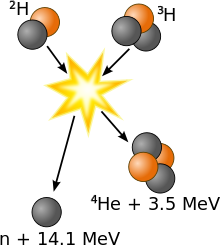
\includegraphics[width=4cm]{fus5}
\caption{A diagram of a Deuterium-Tritium fusion reaction with neutron and helium products \cite{pic}}
\label{fig1}
\end{figure}   
The binding energy of a nucleon is often described as the energy difference between it and the height of the barrier produced by the potential well of the nucleus. When two light nuclei combine together this yields an increase in the binding energy per nucleon, this energy in a fusion process is distributed as kinetic energy among the products of the reaction \cite{text}. The kinetic energy of these products can be collected and harnessed for power.
\section{Discussion}
\subsection{ Physics and Technology conditions for attaining tritium self-sufficiency for the DT fuel cycle \cite{physics}}

\indent \indent This article discusses the importance of tritium breeding in a fusion generator.  It focuses on ITER but the discussion also applies to General Fusion’s reactor. It first talks about the great expense in acquiring an amount of tritium from an outside source that is large enough to sustain a fusion power plant.  This is due to the fact that only trace amounts are found naturally.It then proceeds to examine the production of tritium within a fusion reactor and required production rates.  This article effectively conveys the importance of self-sufficiency when it comes to tritium production for reactor fuel.  It goes into detail about many different components of a potential reactor vessel and the required characteristics of viable materials.  For given materials, this article discusses how each material effects tritium production.  If fusion reactors such as ITER had to rely on current tritium supplies they would exhaust them quickly and the fusion reaction would stop.  For this reason, tritium breeding in the reactor itself is an elegant and effective solution.\newline
\indent The paper mentions that tritium self-sufficiency is complicated because it is affected by all aspects of the fusion system.  This includes the plasma configuration, operation modes and parameters, control systems for plasma stability, heating and exhaust systems embedded, and the blanket and tritium processing systems.  The authors state that “it is clear that tritium self-sufficiency in DT fusion power plants cannot be assured unless specific plasma and technology conditions are met”.  When considering the technological hurdles that must be overcome in order to create a viable fusion reactor, tritium breeding and processing is one of the most significant considerations to make.\newline
\indent The effects of uncertainties in nuclear data are examined because certainty in the rate of tritium production is crucial.  Overall precision in analysis of the reactor conditions before, during and after the actual fusion reaction is imperative. \newline
Another important parameter is the ratio of consumed tritium to the tritium produced.  In order to be self-sufficient, the amount of produced tritium must exceed that of the consumed tritium that was initially in the system.  It is simply not enough to have a 1:1 ratio as some tritium is lost through radioactive decay.  Having excess tritium would also allow for a reserve supply that could be used in the start-up of other reactors or as a back-up for the source reactor.\newline
\indent An interesting aspect of the tritium self-sufficiency potential of a reactor is its dependence on reactor design as it is affected by such things as the breeding blanket coverage and thickness.  For both the ITER and General Fusion reactors there is a neutron absorber between the plasma in the center of the reactor and the breeding blanket on the outside.  This neutron absorbing material has a significant impact on the tritium breeding ratio. The authors investigated this and found that the ratio can decrease by up to 16\% for an increase of 4cm in the thickness of the neutron absorber which emphasizes the effect of reactor design on creating viable fusion.
\newline
 \subsection{Unsolved issues on tritium mass transfer in Li-Pb blankets \cite{unsolved}}
 
\indent \indent This article addresses the viability of a LiPb alloy blanket for use in a fusion reactor.  The LiPb blanket is used in General Fusion’s magnetized Target fusion reactor and is a candidate for use at ITER as a heat exchanger as well as a tritium breeder.  LiPb has a high tritium breeding ratio, appropriate melting point, and low reactivity which makes it a suitable candidate for a liquid first wall inside the reactor.\newline
The paper discusses the importance of knowing the diffusivity of hydrogen, deuterium and tritium within the alloy as well as the wettability between the alloy and the outside surface of the reactor.  If the wettability is unsatisfactory the formation of tritium bubbles between the liquid-solid interface decreases the overall tritium content of the blanket. \newline 
\indent The wettability of the liquid LiPb blanket is an important factor in its usefulness as a blanket material.  For liquids with high surface tension the interface between liquid and, for example, the inside shell of the reactor vessel might not be perfect.  There may be bubbles generated between the two materials which creates the appearance of increased solubility of the hydrogen isotopes.
This paper also examines how impurities in the alloy may affect solubility of hydrogen isotopes (D and T).  The authors discuss the fact that solubility data indicates reactions with oxygen decrease hydrogen solubility and use this as evidence for the importance of oxygen control when implementing a LiPb blanket.\newline
\indent The findings of this paper are that microbubbles at the interface of the LiPb alloy have no effect on the values of permeability, diffusivity and solubility because they are so small.  While there may be a small effect, it is not significant enough to affect the reactor vessel in a noticeable way.\newline
\indent Also discussed is the effect of oxygen inside the reactor vessel.  Because Li can react with oxygen to form Li2O, oxygen control is important when using Li in the fusion blanket.  Reduction of Li concentration would reduce the amount of tritium being bred by the reactor and therefore negatively affect the overall function of the reactor.  The importance of precise knowledge of tritium concentrations is discussed in [A].
\newline




\subsection{An Acoustically Driven Magnetized Target Fusion Reactor \cite{An}}
 

\indent \indent This article compares the most common approach to Magnetized Target Fusion (MTF), with General Fusions acoustically driven MTF reactor.  Usually MTF is done by taking a cold low density fuel, then promptly compressing it to thermonuclear conditions.  The most examined case places the plasma in a conductive metal tube.  Current is then passed through this tube resulting in rapid compression of the plasma.  This process requires constant replacement of components, which Laberge suggests as being quite an expensive drawback. \newline 
\indent In this paper a completely reworked compression system is introduced and Laberge insists offers many advantages.  The basis of the reactor consists of a steel shell surrounded by actuated pistons, and is filled with a liquid lithium lead alloy.  A columnar void is produced inside the sphere by pumping the lead tangentially at its equator.  While plasma is injected and confined in the center of the system, pistons focus acoustic waves rapidly compressing the fuel.  The fuel undergoes fusion, releasing many energetic neutrons which then heat up the lead.  This can be cycled near water to produce steam and furthermore electricity.
\begin{figure}[h!]
\centering
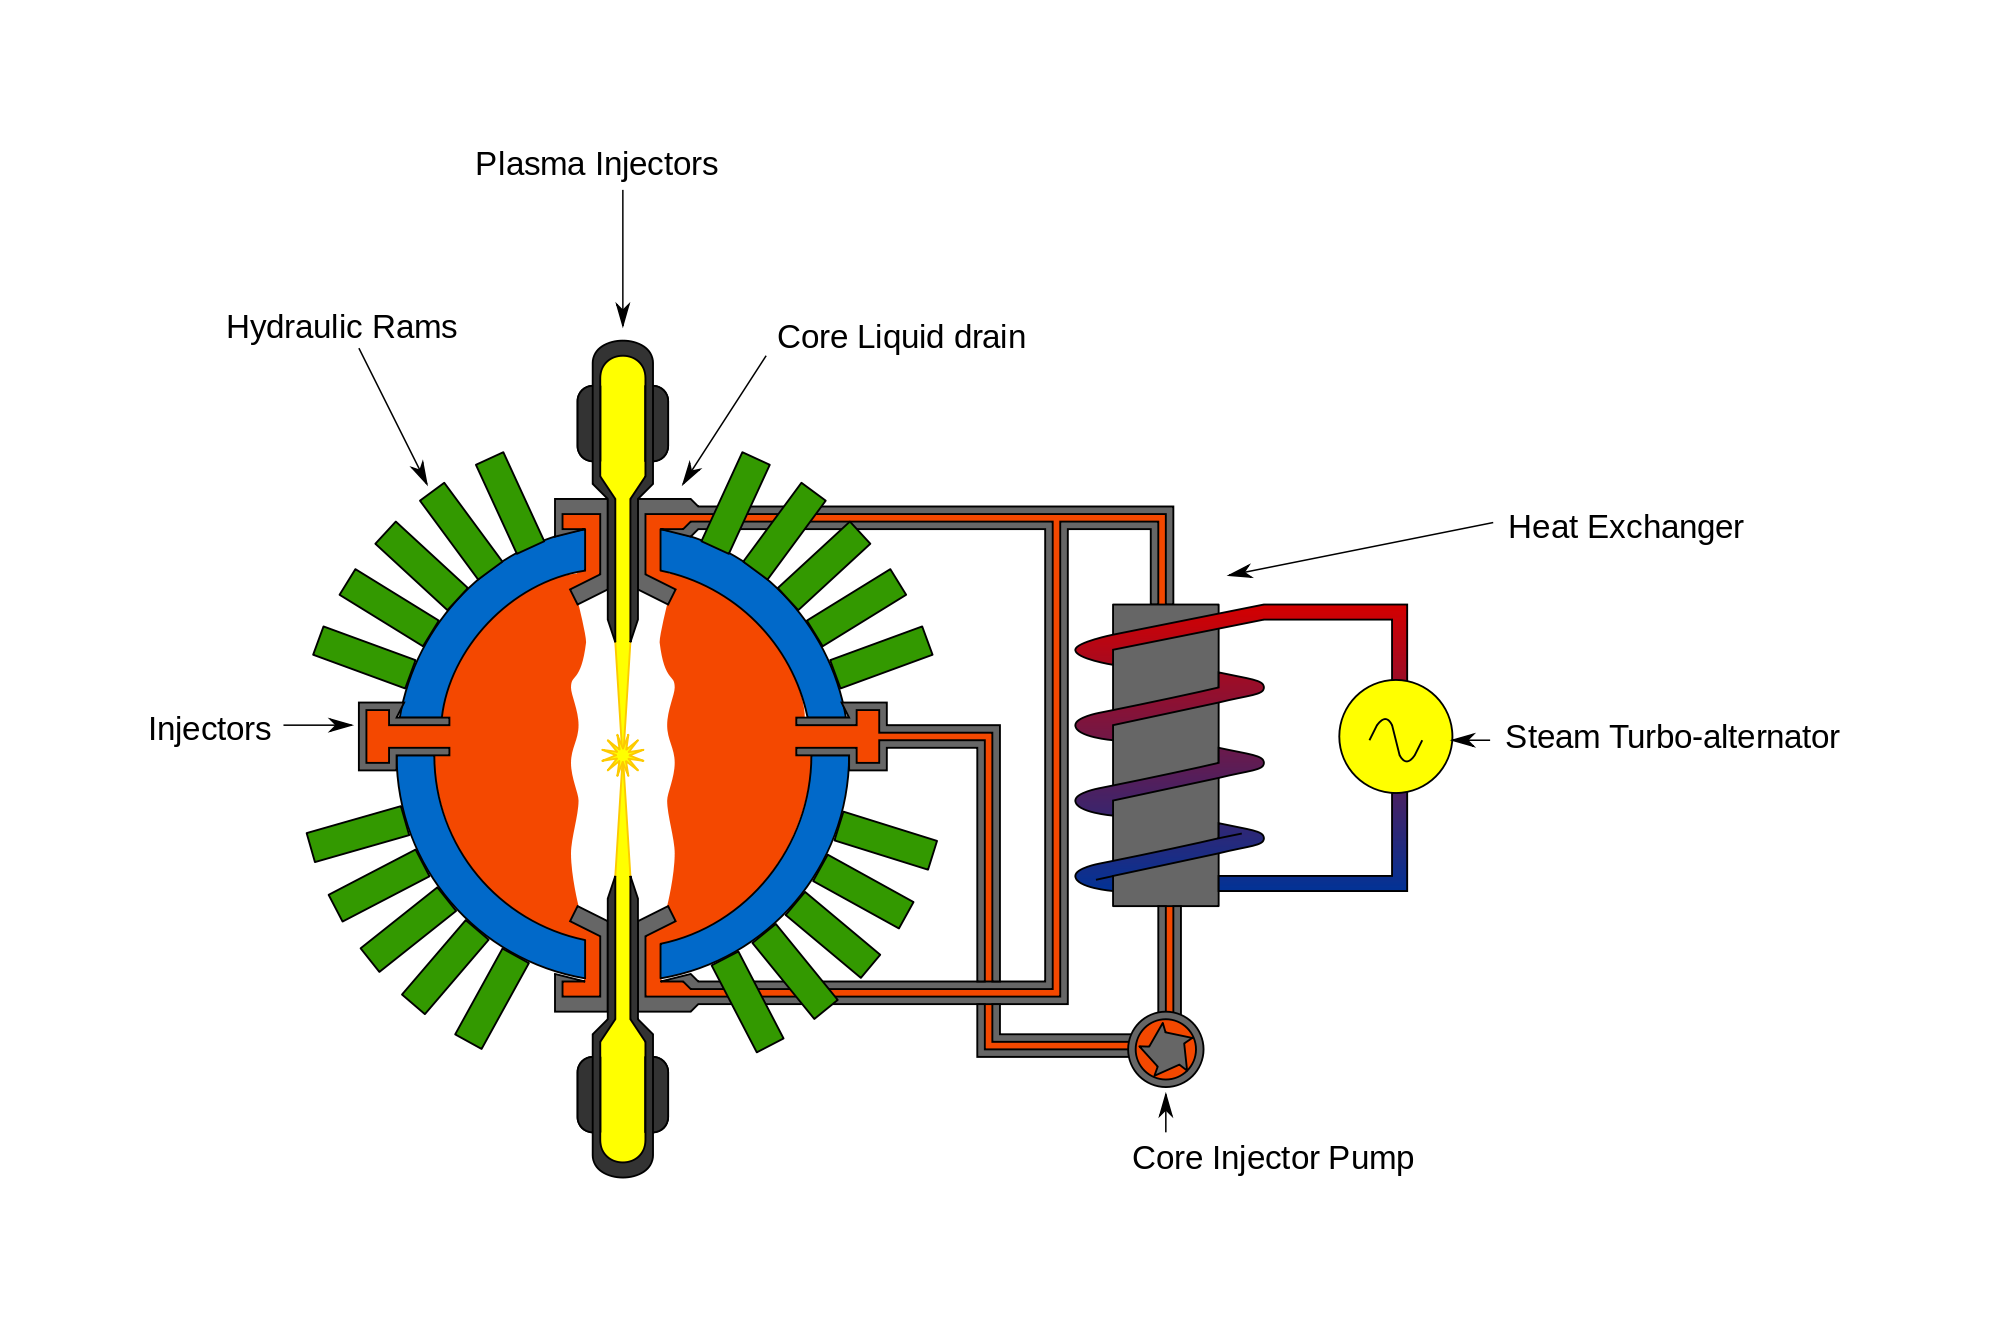
\includegraphics[width=\linewidth]{fus2}
\caption{A simplified schematic of the General Fusion reactor \cite{An}}
\label{fig1}
\end{figure}    
    
\indent  Lithium can easily be employed within the lead alloy to reproduce tritium, a component of the nuclear fuel.  The importance of this rebreeding was discussed in [A].  Another self-sufficient design of the reactor is that the created steam can used to refire the pistons instead of creating electricity.  Laberge also discusses the potential damage that can be caused by neutron flux.  That is, the fusion reaction outputs a large number of energetic neutrons which have the means to harm reactor components.  Furthermore he points out that this design is superb as the entire reaction is surrounded by LiPb, which only allows the neutrons to travel a mere meter before losing most of their kinetic energy. \newline  
\indent The initial experiment that was carried out in this paper in 2009 did not use the same design, but was instead employed as a proof of concept.  Using a totally different method for pressure generation, its goal was to simply produce fusion via pressure waves.  This goal was achieved, as multiple thousands of neutrons were detected after the fuel sources had been compressed.\newline  
\indent General Fusions acoustic MTF reactors require less energy to produce fusion, and minimal maintenance per pulse.  Virtually all aspects of this reactors design reduces cost unlike previous MTF reactors or the massive project ITER.  
\newline


\subsection{Fusion Energy Conversion In Magnetically Confined Plasma Reactors \citep{fusion}}


\indent \indent This paper focuses on the viability of fusion reactions and fuel for the International Thermonuclear Experimental Reactor (ITER).  Although different reactors both ITER and General Fusion require Deuteron-Tritium reactions as their fuel source. \newline 
\indent ITER employs a tokamak reactor which uses magnetic confinement methods to house the fusion reaction. Specially designed magnetic fields can cause charged particles to be trapped. In the tokamak reactor, a gas composed of the fuel source is ionized into a plasma allowing control using magnetic fields and brought up to fusionable temperatures. Energy is harvested through the absorption of neutrons in the shielding and cooling systems.
When two light nuclei combine together an increase in the binding energy per nucleon is seen, which in a fusion process is distributed as kinetic energy among the products of the reaction. The kinetic energy of these products can be collected and harnessed for power.\newline
\indent Dobran explains that the main idea behind high temperature fusion is to replicate fusionable environments in a controlled manner. Generally by raising the thermal energy of the reactants we are increasing the kinetic energy of the interacting particles. As one raises the temperature you raise the kinetic energy of the constituents and ultimately raise the probability of fusion occurring or more specifically, increasing the nucleons ability to climb the coulombic potential barrier which separates nucleons under normal circumstances. However once the fusionable regime is reached raising the temperature doesn't always guarantee efficiency or increased energy output. There is a ‘sweet spot’ where the maximum reaction rates of fusion is attained. This ‘sweet spot’ is significantly lower for D-T reactions as the author explains makes it a favorable fuel source among the first generation of fusion reactors. Dobran explains other reactions such as Deuterium-Deuterium and Deuterium-Helium-4  are theoretically possible, but the higher temperatures required for break-even need technologies that are not yet adequate.\newline
\indent With the benefits of D-T reactions comes the range of technical downfalls. As the author explains D-T reactions release higher energy neutrons, and since neutrons contain no charge they cannot be controlled with the magnetic trap employed by the ITER reactor. This means significant shielding is required to absorb the escaping neutrons and prevent reactor damage. However the escaping neutrons provide an excellent means of harvesting energy without perturbing the plasma. \newline
\indent D-T reactions require a non-abundant fuel source tritium. The author explains tritium breeding using neutron bombardment provides a solution. Both ITER and General Fusion plan to employ liquid and solid shielding/cooling for neutron absorption which can be implanted with lithium for tritium fuel breeding.  Flavio insists the objectives of ITER is to explore the consistency of confining plasma, net energy production, rebreeding tritium for fuel, and the maintainability of the reactor components which will provide valuable research for future reactors.

\section{Conclusion}
\indent \indent Fusion technologies are becoming more viable with passing years, offering a clean solution to an inevitable energy crisis.  Common difficulties with fusion consist of technical confinement and operational costs.  General Fusion proposes relatively simple solutions to these things with an acoustic version of a MTF reactor while ITER attempts to create a somewhat more complicated but equally viable reactor.  Attempts at breaking even in terms of energy have been made, and both companies believe they will go far beyond this.  As research into materials and methods advances, fusion energy technology moves ever closer to the brink of viability.  The construction of both reactors will provide the international community with real-life opportunities to explore the viability of different reactor configurations and materials and will hopefully provide the final push that will result in an energy solution for the future.




\begin{acknowledgements}
      Special thanks goes to Dr. Mark Paetkau who had no involvement. 
\end{acknowledgements}


%-------------------------------------------------------------------

\begin{thebibliography}{}

\bibitem[1]{text} Harms, A. A., Schoepf, K. F., Miley, G.H., and Kingdon, D.R. (2000). "Principles of Fusion Energy." Rosewood Drive, MA. World Scientific Publishing Co. Pte. Ltd 

\bibitem[2]{physics} Sawan M.E. (2006)
"Physics and Technology conditions for attaining tritium self-sufficiency for the DT fuel cycle." Fusion Engineering and Design
[accessed 2014 Feb 2] 81:1131-1144

\bibitem[3]{unsolved} Fukada S, Edao Y. (2011) "Unsolved issues on tritium mass transfer in Li-Pb blankets." Journal of Nuclear Materials. [accessed 2014 Feb 2] 417:727-730. 

\bibitem[4]{An} Laberge, Michel (2009)
"An Acoustically Driven Magnetized Target Fusion Reactor."  AIP Conference Proceedings
7/26/2009, Vol. 1154 Issue 1, p282-288. 7p. 4


\bibitem[5]{fusion} Flavio Dobran (2012)
"Fusion Energy Conversion In Magnetically Confined Plasma Reactors."  Progress In Nuclear Energy
 8/2012, Vol. 60, p89-116
 
 
\bibitem[6]{pic} Wikipedia "Deuterium Tritium Reaction" http://en.wikipedia.org \newline /wiki/Nuclear\_$fusion$ [accessed 2014 April 2]
 

 
\end{thebibliography}

\end{document}

%%%%%%%%%%%%%%%%%%%%%%%%%%%%%%%%%%%%%%%%%%%%%%%%%%%%%%%%%%%%%%
Examples for figures using graphicx
A guide "Using Imported Graphics in LaTeX2e"  (Keith Reckdahl)
is available on a lot of LaTeX public servers or ctan mirrors.
The file is : epslatex.pdf 
%%%%%%%%%%%%%%%%%%%%%%%%%%%%%%%%%%%%%%%%%%%%%%%%%%%%%%%%%%%%%%

%_____________________________________________________________
%                 A figure as large as the width of the column
%-------------------------------------------------------------
   \begin{figure}
   \centering
   \includegraphics[width=\hsize]{empty.eps}
      \caption{Vibrational stability equation of state
               $S_{\mathrm{vib}}(\lg e, \lg \rho)$.
               $>0$ means vibrational stability.
              }
         \label{FigVibStab}
   \end{figure}
%
%_____________________________________________________________
%                                    One column rotated figure
%-------------------------------------------------------------
   \begin{figure}
   \centering
   \includegraphics[angle=-90,width=3cm]{empty.eps}
      \caption{Vibrational stability equation of state
               $S_{\mathrm{vib}}(\lg e, \lg \rho)$.
               $>0$ means vibrational stability.
              }
         \label{FigVibStab}
   \end{figure}
%
%_____________________________________________________________
%                        Figure with caption on the right side 
%-------------------------------------------------------------
   \begin{figure}
   \sidecaption
   \includegraphics[width=3cm]{empty.eps}
      \caption{Vibrational stability equation of state
               $S_{\mathrm{vib}}(\lg e, \lg \rho)$.
               $>0$ means vibrational stability.
              }
         \label{FigVibStab}
   \end{figure}
%
%_____________________________________________________________
%
%_____________________________________________________________
%                                Figure with a new BoundingBox 
%-------------------------------------------------------------
   \begin{figure}
   \centering
   \includegraphics[bb=10 20 100 300,width=3cm,clip]{empty.eps}
      \caption{Vibrational stability equation of state
               $S_{\mathrm{vib}}(\lg e, \lg \rho)$.
               $>0$ means vibrational stability.
              }
         \label{FigVibStab}
   \end{figure}
%
%_____________________________________________________________
%
%_____________________________________________________________
%                                      The "resizebox" command 
%-------------------------------------------------------------
   \begin{figure}
   \resizebox{\hsize}{!}
            {\includegraphics[bb=10 20 100 300,clip]{empty.eps}
      \caption{Vibrational stability equation of state
               $S_{\mathrm{vib}}(\lg e, \lg \rho)$.
               $>0$ means vibrational stability.
              }
         \label{FigVibStab}
   \end{figure}
%
%______________________________________________________________
%
%_____________________________________________________________
%                                             Two column Figure 
%-------------------------------------------------------------
   \begin{figure*}
   \resizebox{\hsize}{!}
            {\includegraphics[bb=10 20 100 300,clip]{empty.eps}
      \caption{Vibrational stability equation of state
               $S_{\mathrm{vib}}(\lg e, \lg \rho)$.
               $>0$ means vibrational stability.
              }
         \label{FigVibStab}
   \end{figure*}
%
%______________________________________________________________
%
%_____________________________________________________________
%                                             Simple A&A Table
%_____________________________________________________________
%
\begin{table}
\caption{Nonlinear Model Results}             % title of Table
\label{table:1}      % is used to refer this table in the text
\centering                          % used for centering table
\begin{tabular}{c c c c}        % centered columns (4 columns)
\hline\hline                 % inserts double horizontal lines
HJD & $E$ & Method\#2 & Method\#3 \\    % table heading 
\hline                        % inserts single horizontal line
   1 & 50 & $-837$ & 970 \\      % inserting body of the table
   2 & 47 & 877    & 230 \\
   3 & 31 & 25     & 415 \\
   4 & 35 & 144    & 2356 \\
   5 & 45 & 300    & 556 \\ 
\hline                                   %inserts single line
\end{tabular}
\end{table}
%
%_____________________________________________________________
%                                             Two column Table 
%_____________________________________________________________
%
\begin{table*}
\caption{Nonlinear Model Results}             
\label{table:1}      
\centering          
\begin{tabular}{c c c c l l l }     % 7 columns 
\hline\hline       
                      % To combine 4 columns into a single one 
HJD & $E$ & Method\#2 & \multicolumn{4}{c}{Method\#3}\\ 
\hline                    
   1 & 50 & $-837$ & 970 & 65 & 67 & 78\\  
   2 & 47 & 877    & 230 & 567& 55 & 78\\
   3 & 31 & 25     & 415 & 567& 55 & 78\\
   4 & 35 & 144    & 2356& 567& 55 & 78 \\
   5 & 45 & 300    & 556 & 567& 55 & 78\\
\hline                  
\end{tabular}
\end{table*}
%
%-------------------------------------------------------------
%                                          Table with notes 
%-------------------------------------------------------------
%
% A single note
\begin{table}
\caption{\label{t7}Spectral types and photometry for stars in the
  region.}
\centering
\begin{tabular}{lccc}
\hline\hline
Star&Spectral type&RA(J2000)&Dec(J2000)\\
\hline
69           &B1\,V     &09 15 54.046 & $-$50 00 26.67\\
49           &B0.7\,V   &*09 15 54.570& $-$50 00 03.90\\
LS~1267~(86) &O8\,V     &09 15 52.787&11.07\\
24.6         &7.58      &1.37 &0.20\\
\hline
LS~1262      &B0\,V     &09 15 05.17&11.17\\
MO 2-119     &B0.5\,V   &09 15 33.7 &11.74\\
LS~1269      &O8.5\,V   &09 15 56.60&10.85\\
\hline
\end{tabular}
\tablefoot{The top panel shows likely members of Pismis~11. The second
panel contains likely members of Alicante~5. The bottom panel
displays stars outside the clusters.}
\end{table}
%
% More notes
%
\begin{table}
\caption{\label{t7}Spectral types and photometry for stars in the
  region.}
\centering
\begin{tabular}{lccc}
\hline\hline
Star&Spectral type&RA(J2000)&Dec(J2000)\\
\hline
69           &B1\,V     &09 15 54.046 & $-$50 00 26.67\\
49           &B0.7\,V   &*09 15 54.570& $-$50 00 03.90\\
LS~1267~(86) &O8\,V     &09 15 52.787&11.07\tablefootmark{a}\\
24.6         &7.58\tablefootmark{1}&1.37\tablefootmark{a}   &0.20\tablefootmark{a}\\
\hline
LS~1262      &B0\,V     &09 15 05.17&11.17\tablefootmark{b}\\
MO 2-119     &B0.5\,V   &09 15 33.7 &11.74\tablefootmark{c}\\
LS~1269      &O8.5\,V   &09 15 56.60&10.85\tablefootmark{d}\\
\hline
\end{tabular}
\tablefoot{The top panel shows likely members of Pismis~11. The second
panel contains likely members of Alicante~5. The bottom panel
displays stars outside the clusters.\\
\tablefoottext{a}{Photometry for MF13, LS~1267 and HD~80077 from
Dupont et al.}
\tablefoottext{b}{Photometry for LS~1262, LS~1269 from
Durand et al.}
\tablefoottext{c}{Photometry for MO2-119 from
Mathieu et al.}
}
\end{table}
%
%-------------------------------------------------------------
%                                       Table with references 
%-------------------------------------------------------------
%
\begin{table*}[h]
 \caption[]{\label{nearbylistaa2}List of nearby SNe used in this work.}
\begin{tabular}{lccc}
 \hline \hline
  SN name &
  Epoch &
 Bands &
  References \\
 &
  (with respect to $B$ maximum) &
 &
 \\ \hline
1981B   & 0 & {\it UBV} & 1\\
1986G   &  $-$3, $-$1, 0, 1, 2 & {\it BV}  & 2\\
1989B   & $-$5, $-$1, 0, 3, 5 & {\it UBVRI}  & 3, 4\\
1990N   & 2, 7 & {\it UBVRI}  & 5\\
1991M   & 3 & {\it VRI}  & 6\\
\hline
\noalign{\smallskip}
\multicolumn{4}{c}{ SNe 91bg-like} \\
\noalign{\smallskip}
\hline
1991bg   & 1, 2 & {\it BVRI}  & 7\\
1999by   & $-$5, $-$4, $-$3, 3, 4, 5 & {\it UBVRI}  & 8\\
\hline
\noalign{\smallskip}
\multicolumn{4}{c}{ SNe 91T-like} \\
\noalign{\smallskip}
\hline
1991T   & $-$3, 0 & {\it UBVRI}  &  9, 10\\
2000cx  & $-$3, $-$2, 0, 1, 5 & {\it UBVRI}  & 11\\ %
\hline
\end{tabular}
\tablebib{(1)~\citet{branch83};
(2) \citet{phillips87}; (3) \citet{barbon90}; (4) \citet{wells94};
(5) \citet{mazzali93}; (6) \citet{gomez98}; (7) \citet{kirshner93};
(8) \citet{patat96}; (9) \citet{salvo01}; (10) \citet{branch03};
(11) \citet{jha99}.
}
\end{table}
%_____________________________________________________________
%                      A rotated Two column Table in landscape  
%-------------------------------------------------------------
\begin{sidewaystable*}
\caption{Summary for ISOCAM sources with mid-IR excess 
(YSO candidates).}\label{YSOtable}
\centering
\begin{tabular}{crrlcl} 
\hline\hline             
ISO-L1551 & $F_{6.7}$~[mJy] & $\alpha_{6.7-14.3}$ 
& YSO type$^{d}$ & Status & Comments\\
\hline
  \multicolumn{6}{c}{\it New YSO candidates}\\ % To combine 6 columns into a single one
\hline
  1 & 1.56 $\pm$ 0.47 & --    & Class II$^{c}$ & New & Mid\\
  2 & 0.79:           & 0.97: & Class II ?     & New & \\
  3 & 4.95 $\pm$ 0.68 & 3.18  & Class II / III & New & \\
  5 & 1.44 $\pm$ 0.33 & 1.88  & Class II       & New & \\
\hline
  \multicolumn{6}{c}{\it Previously known YSOs} \\
\hline
  61 & 0.89 $\pm$ 0.58 & 1.77 & Class I & \object{HH 30} & Circumstellar disk\\
  96 & 38.34 $\pm$ 0.71 & 37.5& Class II& MHO 5          & Spectral type\\
\hline
\end{tabular}
\end{sidewaystable*}
%_____________________________________________________________
%                      A rotated One column Table in landscape  
%-------------------------------------------------------------
\begin{sidewaystable}
\caption{Summary for ISOCAM sources with mid-IR excess 
(YSO candidates).}\label{YSOtable}
\centering
\begin{tabular}{crrlcl} 
\hline\hline             
ISO-L1551 & $F_{6.7}$~[mJy] & $\alpha_{6.7-14.3}$ 
& YSO type$^{d}$ & Status & Comments\\
\hline
  \multicolumn{6}{c}{\it New YSO candidates}\\ % To combine 6 columns into a single one
\hline
  1 & 1.56 $\pm$ 0.47 & --    & Class II$^{c}$ & New & Mid\\
  2 & 0.79:           & 0.97: & Class II ?     & New & \\
  3 & 4.95 $\pm$ 0.68 & 3.18  & Class II / III & New & \\
  5 & 1.44 $\pm$ 0.33 & 1.88  & Class II       & New & \\
\hline
  \multicolumn{6}{c}{\it Previously known YSOs} \\
\hline
  61 & 0.89 $\pm$ 0.58 & 1.77 & Class I & \object{HH 30} & Circumstellar disk\\
  96 & 38.34 $\pm$ 0.71 & 37.5& Class II& MHO 5          & Spectral type\\
\hline
\end{tabular}
\end{sidewaystable}
%
%_____________________________________________________________
%                              Table longer than a single page  
%-------------------------------------------------------------
% All long tables will be placed automatically at the end, after 
%                                        \end{thebibliography}
%
\begin{longtab}
\begin{longtable}{lllrrr}
\caption{\label{kstars} Sample stars with absolute magnitude}\\
\hline\hline
Catalogue& $M_{V}$ & Spectral & Distance & Mode & Count Rate \\
\hline
\endfirsthead
\caption{continued.}\\
\hline\hline
Catalogue& $M_{V}$ & Spectral & Distance & Mode & Count Rate \\
\hline
\endhead
\hline
\endfoot
%%
Gl 33    & 6.37 & K2 V & 7.46 & S & 0.043170\\
Gl 66AB  & 6.26 & K2 V & 8.15 & S & 0.260478\\
Gl 68    & 5.87 & K1 V & 7.47 & P & 0.026610\\
         &      &      &      & H & 0.008686\\
Gl 86 
\footnote{Source not included in the HRI catalog. See Sect.~5.4.2 for details.}
         & 5.92 & K0 V & 10.91& S & 0.058230\\
\end{longtable}
\end{longtab}
%
%_____________________________________________________________
%                              Table longer than a single page
%                                             and in landscape 
%  In the preamble, use:       \usepackage{lscape}
%-------------------------------------------------------------
% All long tables will be placed automatically at the end, after
%                                        \end{thebibliography}
%
\begin{longtab}
\begin{landscape}
\begin{longtable}{lllrrr}
\caption{\label{kstars} Sample stars with absolute magnitude}\\
\hline\hline
Catalogue& $M_{V}$ & Spectral & Distance & Mode & Count Rate \\
\hline
\endfirsthead
\caption{continued.}\\
\hline\hline
Catalogue& $M_{V}$ & Spectral & Distance & Mode & Count Rate \\
\hline
\endhead
\hline
\endfoot
%%
Gl 33    & 6.37 & K2 V & 7.46 & S & 0.043170\\
Gl 66AB  & 6.26 & K2 V & 8.15 & S & 0.260478\\
Gl 68    & 5.87 & K1 V & 7.47 & P & 0.026610\\
         &      &      &      & H & 0.008686\\
Gl 86
\footnote{Source not included in the HRI catalog. See Sect.~5.4.2 for details.}
         & 5.92 & K0 V & 10.91& S & 0.058230\\
\end{longtable}
\end{landscape}
\end{longtab}
%
% Online Material
%_____________________________________________________________
%        Online appendices have to be placed at the end, after
%                                        \end{thebibliography}
%-------------------------------------------------------------
\end{thebibliography}

\Online

\begin{appendix} %First online appendix
\section{Background galaxy number counts and shear noise-levels}
Because the optical images used in this analysis...

\begin{figure*}
\centering
\includegraphics[width=16.4cm,clip]{1787f24.ps}
\caption{Plotted above...}
\label{appfig}
\end{figure*}

Because the optical images...
\end{appendix}

\begin{appendix} %Second online appendix
These studies, however, have faced...
\end{appendix}

\end{document}
%
%_____________________________________________________________
%        Some tables or figures are in the printed version and
%                      some are only in the electronic version
%-------------------------------------------------------------
%
% Leave all the tables or figures in the text, at their right place 
% and use the commands \onlfig{} and \onltab{}. These elements
% will be automatically placed at the end, in the section
% Online material.

\documentclass{aa}
...
\begin{document}
text of the paper...
\begin{figure*}%f1
\includegraphics[width=10.9cm]{1787f01.eps}
\caption{Shown in greyscale is a...}
\label{cl12301}}
\end{figure*}
...
from the intrinsic ellipticity distribution.
% Figure 2 available electronically only
\onlfig{
\begin{figure*}%f2
\includegraphics[width=11.6cm]{1787f02.eps}
\caption {Shown in greyscale...}
\label{cl1018}
\end{figure*}
}

% Figure 3 available electronically only
\onlfig{
\begin{figure*}%f3
\includegraphics[width=11.2cm]{1787f03.eps}
\caption{Shown in panels...}
\label{cl1059}
\end{figure*}
}

\begin{figure*}%f4
\includegraphics[width=10.9cm]{1787f04.eps}
\caption{Shown in greyscale is...}
\label{cl1232}}
\end{figure*}

\begin{table}%t1
\caption{Complexes characterisation.}\label{starbursts}
\centering
\begin{tabular}{lccc}
\hline \hline
Complex & $F_{60}$ & 8.6 &  No. of  \\
...
\hline
\end{tabular}
\end{table}
The second method produces...

% Figure 5 available electronically only
\onlfig{
\begin{figure*}%f5
\includegraphics[width=11.2cm]{1787f05.eps}
\caption{Shown in panels...}
\label{cl1238}}
\end{figure*}
}

As can be seen, in general the deeper...
% Table 2 available electronically only
\onltab{
\begin{table*}%t2
\caption{List of the LMC stellar complexes...}\label{Properties}
\centering
\begin{tabular}{lccccccccc}
\hline  \hline
Stellar & RA & Dec & ...
...
\hline
\end{tabular}
\end{table*}
}

% Table 3 available electronically only
\onltab{
\begin{table*}%t3
\caption{List of the derived...}\label{IrasFluxes}
\centering
\begin{tabular}{lcccccccccc}
\hline \hline
Stellar & $f12$ & $L12$ &...
...
\hline
\end{tabular}
\end{table*}
}
%
%-------------------------------------------------------------
%     For the online material, table longer than a single page
%                 In the preamble for landscape case, use : 
%                                          \usepackage{lscape}
%-------------------------------------------------------------
\documentclass{aa}
\usepackage[varg]{txfonts}
\usepackage{graphicx}
\usepackage{lscape}

\begin{document}
text of the paper
% Table will be print automatically at the end, in the section Online material.
\onllongtab{
\begin{longtable}{lrcrrrrrrrrl}
\caption{Line data and abundances ...}\\
\hline
\hline
Def & mol & Ion & $\lambda$ & $\chi$ & $\log gf$ & N & e &  rad & $\delta$ & $\delta$ 
red & References \\
\hline
\endfirsthead
\caption{Continued.} \\
\hline
Def & mol & Ion & $\lambda$ & $\chi$ & $\log gf$ & B & C &  rad & $\delta$ & $\delta$ 
red & References \\
\hline
\endhead
\hline
\endfoot
\hline
\endlastfoot
A & CH & 1 &3638 & 0.002 & $-$2.551 &  &  &  & $-$150 & 150 &  Jorgensen et al. (1996) \\                    
\end{longtable}
}% End onllongtab

% Or for landscape, large table:

\onllongtab{
\begin{landscape}
\begin{longtable}{lrcrrrrrrrrl}
...
\end{longtable}
\end{landscape}
}% End onllongtab
